\documentclass[10pt, landscape]{article}
\usepackage[scaled=0.92]{helvet}
\usepackage{calc}
\usepackage{multicol}
\usepackage{ifthen}
\usepackage[a4paper,margin=5mm,landscape]{geometry}
\usepackage{amsmath,amsthm,amsfonts,amssymb}
\usepackage{color,graphicx,overpic}
\usepackage{hyperref}
\usepackage{newtxtext} 
\usepackage{enumitem}
\usepackage{amssymb}
\usepackage[table]{xcolor}
\usepackage{vwcol}
\usepackage{tikz}
\usetikzlibrary{arrows.meta}
\usetikzlibrary{calc}
\usepackage{mathtools}
\usepackage{nicematrix}
\usepackage[T1]{fontenc} %%% <--- NOTE THIS
% for relations
\usepackage{cancel}
\usepackage{ mathrsfs }
\usepackage{listings}
\usepackage{background}
\setlist{nosep}

\usepackage{etoolbox}
\makeatletter
\preto{\@verbatim}{\topsep=0pt \partopsep=0pt }
\makeatother

\backgroundsetup{
scale=1,
color=black,
opacity=0.4,
angle=0,
contents={%
  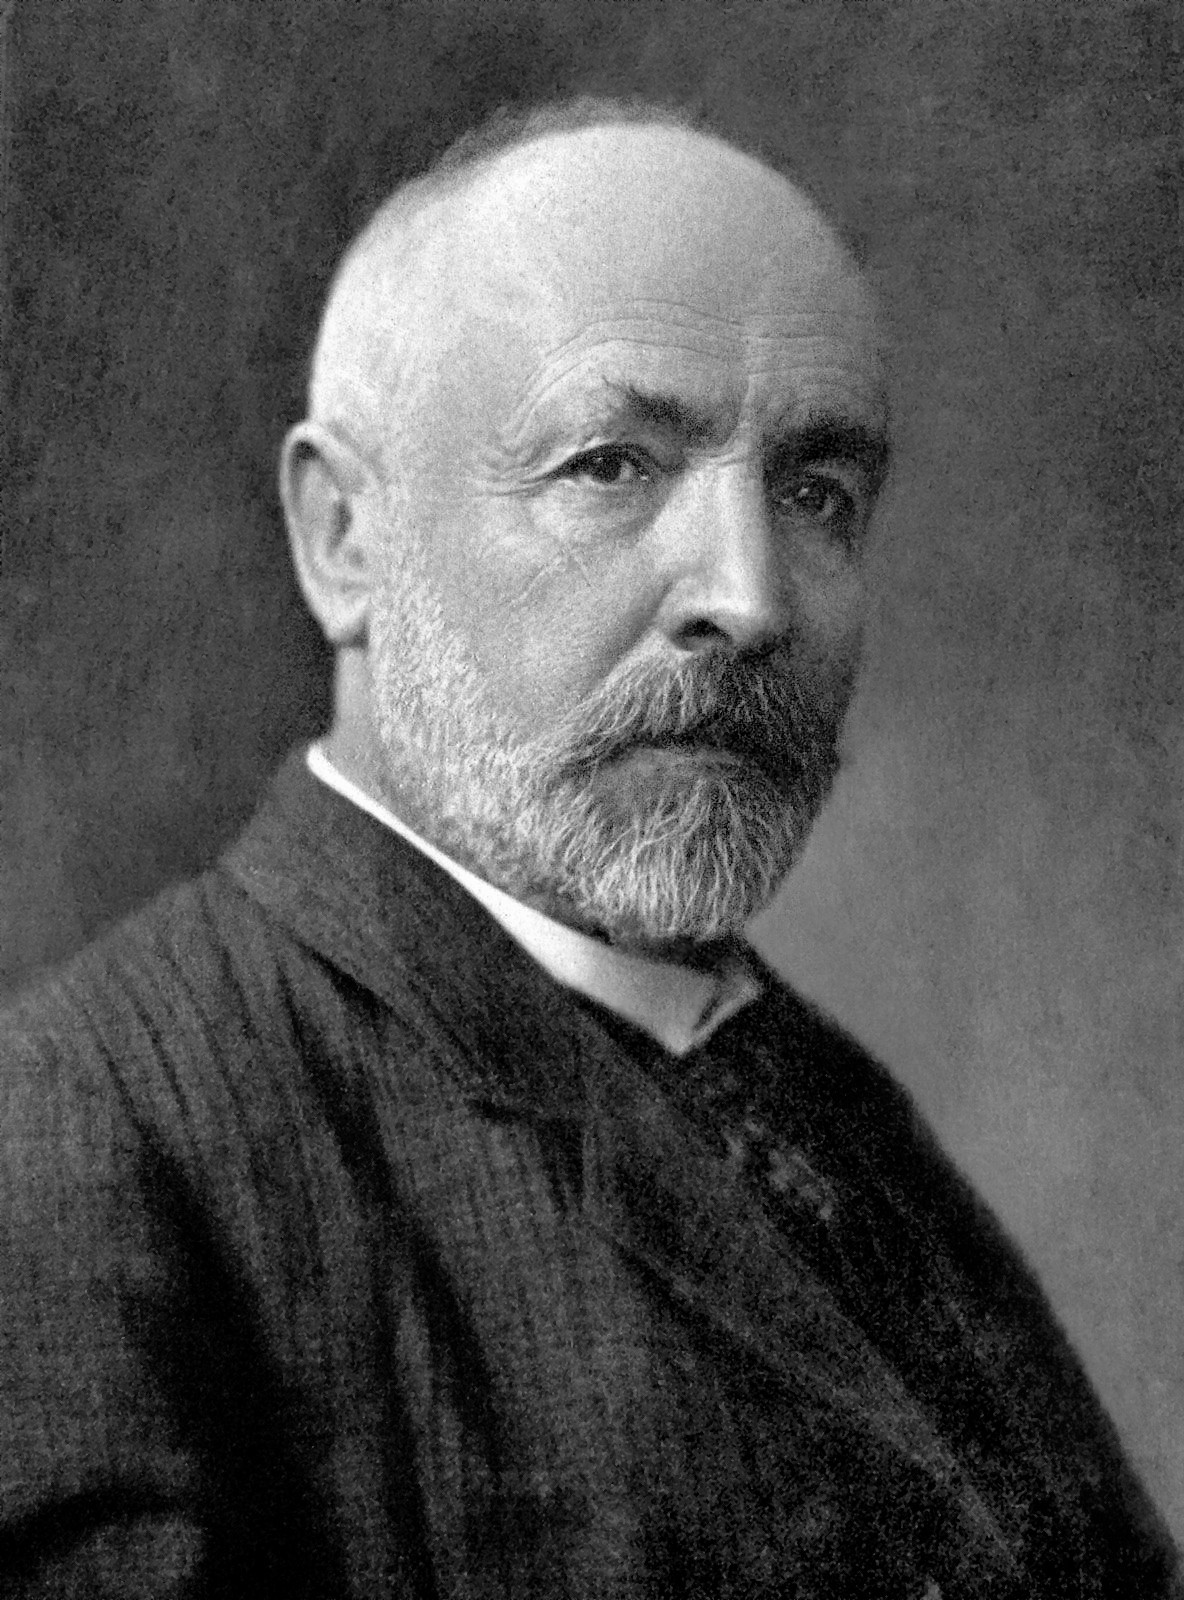
\includegraphics[width=0.5\paperwidth,height=\paperheight]{cantor.jpg}
  
\includegraphics[width=0.5\paperwidth,height=\paperheight]{dilip.jpg}
  }%
}

\pdfinfo{
  /Title (MA3205.pdf)
  /Creator (TeX)
  /Producer (pdfTeX 1.40.0)
  /Author (Seamus)
  /Subject (Example)
  /Keywords (pdflatex, latex,pdftex,tex)}

\lstset{language=Java,keywordstyle={\bfseries \color{black}}}

% Turn off header and footer
\pagestyle{empty}

\newenvironment{tightcenter}{%
  \setlength\topsep{0pt}
  \setlength\parskip{0pt}
  \begin{center}
}{%
  \end{center}
}

% redefine section commands to use less space
\makeatletter
\renewcommand{\section}{\@startsection{section}{1}{0mm}%
                                {-1ex plus -.5ex minus -.2ex}%
                                {0.5ex plus .2ex}%x
                                {\normalfont\large\bfseries}}
\renewcommand{\section}{\@startsection{section}{2}{0mm}%
                                {-1explus -.5ex minus -.2ex}%
                                {0.5ex plus .2ex}%
                                {\normalfont\normalsize\bfseries}}
\renewcommand{\subsection}{\@startsection{subsection}{3}{0mm}%
                                {-1ex plus -.5ex minus -.2ex}%
                                {1ex plus .2ex}%
                                {\normalfont\small\bfseries}}%
\renewcommand{\familydefault}{\sfdefault}
\renewcommand\rmdefault{\sfdefault}
% makes nested numbering (e.g. 1.1.1, 1.1.2, etc)
\renewcommand{\labelenumii}{\theenumii}
\renewcommand{\theenumii}{\theenumi.\arabic{enumii}.}
\renewcommand\labelitemii{•}
%  for logical not operator
\renewcommand{\lnot}{\mathord{\sim}}
\renewcommand{\bf}[1]{\textbf{#1}}
\newcommand{\abs}[1]{\vert #1 \vert}
\newcommand{\Mod}[1]{\ \mathrm{mod}\ #1}

\makeatother
\definecolor{myblue}{cmyk}{1,.72,0,.38}
\everymath\expandafter{\the\everymath \color{myblue}}
% Define BibTeX command
\def\BibTeX{{\rm B\kern-.05em{\sc i\kern-.025em b}\kern-.08em
    T\kern-.1667em\lower.7ex\hbox{E}\kern-.125emX}}
\let\iff\leftrightarrow
\let\Iff\Leftrightarrow
\let\then\rightarrow
\let\Then\Rightarrow

% Don't print section numbers
\setcounter{secnumdepth}{0}

\setlength{\parindent}{0pt}
\setlength{\parskip}{0pt plus 0.5ex}
%% this changes all items (enumerate and itemize)
\setlength{\leftmargini}{0.5cm}
\setlength{\leftmarginii}{0.5cm}
\setlist[itemize,1]{leftmargin=2mm,labelindent=1mm,labelsep=1mm}
\setlist[itemize,2]{leftmargin=4mm,labelindent=1mm,labelsep=1mm}

%My Environments
\newtheorem{example}[section]{Example}
% -----------------------------------------------------------------------

\begin{document}
\raggedright
\footnotesize
\begin{multicols*}{3}

% multicol parameters
% These lengths are set only within the two main columns
\setlength{\columnseprule}{0.25pt}
\setlength{\premulticols}{1pt}
\setlength{\postmulticols}{1pt}
\setlength{\multicolsep}{1pt}
\setlength{\columnsep}{2pt}

\begin{center}
    \fbox{%
        \parbox{0.8\linewidth}{\centering \textcolor{black}{
            {\Large\textbf{MA3205}}
            \\ \normalsize{AY24/25 Sem 2}}
            \\ {\footnotesize \textcolor{myblue}{by ngmh}} 
        }%
    }
\end{center}

\section{Chapter 2 - 8}
\textbf{EP2.36} There is a bijection $F:\mathcal{P}(X)\rightarrow \{0,1\}^X$. 
$F(a)(x) =
    \left\{
    \begin{array}{lr}
      0 & \text{if $x \in A$} \\
      1 & \text{if $x \notin A$} \\
    \end{array}
    \right.
$ which is $1-1$ and onto.

\textbf{D2.37 Cartesian Product} Let $F$ be a function with $dom(F)$ as a set. $\prod F=\{f:f \ \text{is a function} \land dom(f) = dom(F) \land \forall x \in dom(F) \ [f(x) \in F(x)]\}$. If $F=\langle A_i : i \in I \rangle$, then $\prod F = \prod_{i \in I}A_i = \{f: f \ \text{is a function} \land dom(f)=I \land \forall i \in I\ [f(i) \in A_i]\}$

\textbf{A2.38 Axiom of Choice} If $\langle A_i : i \in I \rangle$ is a sequence of sets such that $\forall i \in I \ [A_i \neq \emptyset]$, then $\prod_{i \in I} A_i \neq \emptyset$

\textbf{T5.11 Schröder-Bernstein} If $A \lessapprox B$ and $B \lessapprox A$, then $A \approx B$.

\textbf{D5.19} A set is finite if there exits $n \in \mathbb{N}$ such that $n \approx A$. $A$ is infinite if it is not finite. $A$ is countable if $A \lessapprox \mathbb{N}$. $A$ is uncountable if it is not countable.

\textbf{D6.45/13 Partial/Linear/Well Order}
\begin{enumerate}
    \item $\forall x \in X \ [x \not < x]$
    \item $\forall x, y, z \in X \ [(x < y \land y < z) \Rightarrow x < z]$
    \item $\forall x, y \in X \ [x = y \lor x \lhd y \lor y \lhd x]$ (linear order)
    \item $\forall A \subseteq X \ [A \neq \emptyset \Rightarrow \exists a \in A \ \forall a' \in A \ [a \leq a']]$ (well order)
\end{enumerate}

\textbf{D6.9 Maximal / Minimal Element} $x \in X$ is maximal if $\forall y \in X \ [x \not < y]$.

\textbf{D6.11} $C \subseteq X$ is a chain if $\forall x, y \in C \ [x \text{ and } y \text{ are comparable}]$. $A \subseteq X$ is an antichain if $\forall x, y \in A \ [x \neq y \Rightarrow x \text{ and } y \text{ are incomparable}]$. A chain is maximal if there is no chain $C' \subseteq X$ where $C \subsetneq C'$. $\emptyset$ and singletons are chains and antichains.

\textbf{L6.12} For a finite partial order, every chain or antichain is contained in a maximal chain or antichain.
 
\textbf{D6.16} For a linear order $\langle X, < \rangle$ $pred_{\langle X, < \rangle}(x)=\{x' \in X : x' < x\}$, or the set of predecessors of $x$ in $X$ for the ordering $<$. A subset $A \subseteq X$ is downwards closed if $\forall a \in A \ \forall x \in X \ [x < a \Rightarrow x \in A]$. The predecessor subset is downwards closed along with the entire set.

\textbf{D6.33/34} If $\langle X, \lhd \rangle$ and $\langle Y, \prec \rangle$ are linear orders, $f: X \rightarrow Y$ is an isomorphism between them if $f$ is ($1-1$ and) onto and $\forall x, y \in X \ [x \lhd y \Leftrightarrow f(x) \prec f(y)]$. Two linear orders are isomorphic if $f$ exists which is an isomorphism.

\textbf{D6.35} $\langle X, < \rangle$ and $\langle Y, \prec \rangle$ are linear orders. $f:X\rightarrow Y$ is an embedding it is $1-1$ and order preserving.  $\langle X, <\rangle \hookrightarrow \langle Y, \prec \rangle$.

\textbf{D6.42} A linear order $\langle X, \lhd \rangle$ has type omega $\omega$ if $X$ is infinite and $\forall x \in X$, $pred_{\langle X, \lhd \rangle}(x)$ is finite.

\textbf{L7.6 (AC)} A countable union of countable sets is countable.

\textbf{L7.8} $\mathbb{Q} \approx \mathbb{N}$.

\textbf{F7.12} If $x, y \in \mathbb{R}$ and $x < y$, there is a $q \in \mathbb{Q}$ with $x < q < y$.

\textbf{T7.14/15} $\approx$: $2^\mathbb{N}$, $\mathbb{N}^\mathbb{N}$, $\mathcal{P}(\mathbb{N} \times \mathbb{N})$, $\mathcal{P}(\mathbb{N})$, $\mathcal{P}(\mathbb{Q})$, $\mathbb{R}$, $\mathfrak{c}$, $\mathbb{R}^2$ $\mathbb{R}^\mathbb{N}$.

\textbf{C7.24} If $B \approx C$, then $A^B \approx A^C$.

\textbf{C7.25} If $A \lessapprox D$, $B \lessapprox C$, and $B \neq \emptyset$, then $A^B \lessapprox D^C$.

\textbf{L7.27} Suppose $A$, $B$, and $C$ are sets with $B \cap C = \emptyset$. $A^B \times A^C \approx A^{B \cup C}$.

\textbf{C7.28} $\mathbb{N}^\mathbb{N} \times \mathbb{N}^\mathbb{N} \approx \mathbb{N}^\mathbb{N}$ using $A \cup B = \mathbb{N}, A \cap B = \emptyset$.

\textbf{L7.31/32} Let $A$, $B$, $C$ be sets. $A^{(B \times C)}\approx (A^B)^C$. $(\mathbb{N}^\mathbb{N})^\mathbb{N}\approx \mathbb{N}^\mathbb{N}$.

\textbf{E7.37} $\mathbb{R}^\mathbb{R}\approx 2^\mathbb{R}$.

\textbf{E7.39} There are only $\mathfrak{c}$ many increasing functions.

\textbf{D8.8} Let $\langle X, < \rangle$ be a partial order and $A \subseteq X$. $x \in X$ is an upper bound of $A$ if $\forall a \in A \ [a \leq x]$. $x$ is a lower bound if $\forall a \in A \ [x \leq a]$. Let $U$ be the set of upper bounds of $A$ and $L$ be the set of lower bounds of $A$. If there exists $u \in U$ such that $\forall x \in U \ [u \leq x]$, then $u$ is the supremum of $A$ in $X$ or $sup_X(A)$ or minimal upper bound. For $L$ and $[x \leq l]$, it is called the infimum or $inf_X(A)$ or greatest lower bound. There can only be at most one supremum or infimum.

\textbf{D8.13} A linear order $\langle X, < \rangle$ is dense if $\forall x, y \in X \ \exists z \in X \ [x < y \Rightarrow x < z < y]$.

\textbf{D8.14} A linear order is without endpoints if it has neither a maximal nor minimal element. A countable dense linear order with no endpoints is universal for all countable linear orders; every countable linear order embeds into such an order.

\textbf{T8.15 (Cantor, AC)} Suppose $\langle X, < \rangle$ is a non-empty dense linear order without endpoints. Let $\langle Y, \prec \rangle$ be any countable linear order. Then $\langle Y, \prec \rangle \hookrightarrow \langle X, < \rangle$.

\textbf{T8.16 (Cantor)} Let $\langle X, < \rangle$ and $\langle Y, \prec \rangle$ be non-empty countable dense linear orders without endpoints. Then they are isomorphic.

\section{9. Well-Ordered Sets}
\textbf{F9.1} If $\langle X, < \rangle$ is a linear order of type $\omega$, then it is a well-order.

\textbf{L9.2} Suppose $A$ and $B$ are downwards closed subsert of $X$ where $\langle X, < \rangle$ is a well-order. If $\langle A, <\rangle\cong\langle B, <\rangle$, then $A=B$.

\textbf{C9.3} Suppose $\langle X, < \rangle$ is a well-order, and $x<x'\in X$. Then $\langle pred_{\langle X, < \rangle}(x'), <\rangle \not\cong \langle pred_{\langle X, < \rangle}(x), <\rangle$.

\textbf{C9.4} Suppose $\langle X, <\rangle$ is a well-order. Then for any $x \in X$, $\langle pred_{\langle X, < \rangle}(x), <\rangle \not \cong \langle X, < \rangle$.

\textbf{L9.5} If $\langle X, < \rangle$ and $\langle Y, \prec \rangle$ are isomorphic well-orders, then the isomorphism between them is unique.

\textbf{T9.6} Suppose $\langle X, < \rangle$ and $\langle Y, \prec \rangle$ are well-orders. Then exactly one of the following holds:
\begin{enumerate}
    \item $\langle X, < \rangle \cong \langle Y, \prec \rangle$
    \item $\exists x \in X\ [\langle pred_{\langle X, <\rangle}(x),< \rangle \cong \langle Y, \prec \rangle]$
    \item $\exists y \in Y\ [\langle X, < \rangle \cong \langle pred_{\langle Y, \prec\rangle}(y),\prec \rangle]$
\end{enumerate}

\textbf{E9.11} Define the product of $X$ and $Y$ to be $Z=Y \times X$. The dictionary order $\lhd$ on $Z$ is a well-order.

\textbf{E9.13} Given well-orders $\langle X, <_X \rangle \cong \langle A, <_A \rangle, \langle Y, <_Y \rangle \cong \langle B, <_B \rangle$, then the product and sum of $\langle X, <_X \rangle, \langle Y, <_Y \rangle \cong \langle A, <_A \rangle, \langle B, <_B \rangle$.

\section{10. Ordinals}
$\mathbf{WO}=\{\langle X, <\rangle : X \text{ is a set }\land<\text{is a well-ordering of }X\}$
\subsection{10.1 Basic Properties of Ordinals}
\textbf{D10.1} A set $x$ is transitive if every element of $x$ is a subset of $x$, or $\forall y \ [y \in x \Rightarrow y \subseteq x]$.

\textbf{D10.2 Ordinals} A set $\alpha$ is an ordinal if it is transitive and well-ordered by $\in$. Let $\in_{\alpha}=\{\langle \beta, \gamma \rangle \in \alpha \times \alpha : \beta \in \gamma\}$. $\alpha$ is an ordinal if $\alpha$ is transitive and $\langle \alpha, \in_{\alpha}\rangle$ is a well-order. The subscript of $\in_\alpha$ is often omitted.

\textbf{F10.3} $\mathbb{N}$ is an ordinal. Every $n \in \mathbb{N}$ is also an ordinal.

\textbf{T10.4} Let $x$ be an ordinal. The following hold:
\begin{enumerate}
    \item $\forall y \in x\ [y \text{ is an ordinal} \land y=pred_{\langle x, \in \rangle}(y)]$
    \item if $y$ is any ordinal and $\langle x,\in\rangle \cong \langle y, \in \rangle$ then $x=y$
    \item if $y$ is any ordinal, then exactly one of the following things hold: $x \in y, x=y, y \in x$
    \item if $y, z$ are ordinals and $x\in y$ and $y \in z$, then $x \in z$
    \item if $\mathbf{C}$ is a non-empty class of ordinals, then $\exists y \in \mathbf{C}\ \forall z \in \mathbf{C}\ [y \in z \lor y =z]$
\end{enumerate}

\textbf{D10.5} $\mathbf{ORD}=\{\alpha:\alpha \text{ is an ordinal}\}$ is the class of all ordinals.

\textbf{T10.6 Burali-Forti} $\mathbf{ORD}$ is not a set.

\textbf{L10.7} Every transitive set of ordinals is an ordinal.

\textbf{T10.8} Let $\langle X, < \rangle$ be a well-ordered set. Then there exists a unique $\alpha$ such that $\langle X,<\rangle\cong\langle\alpha, \in_\alpha\rangle$.

\textbf{D10.11} If $\langle X, <\rangle$ is any well-ordered set, then $otp(\langle X, < \rangle)$, or the order type of $\langle X, < \rangle$ is the unique ordinal $\alpha$ such that $\langle X, <\rangle$ is isomorphic to $\langle \alpha, \in_\alpha\rangle$.

\textbf{L10.13} For ordinals $\alpha, \beta$, $\alpha \leq \beta$ iff $\alpha \subseteq \beta$.

\textbf{L10.14} If $A$ is a non-empty set of ordinals, then $min(A)=\bigcap A$. If $A$ is any set of ordinals, then $sup_{\mathbf{ORD}}(A)=\bigcup A$.

\textbf{L10.15} For any $\alpha$, $S(\alpha)$ is an ordinal, $\alpha < S(\alpha)$, and $\forall\beta\ [\beta<S(\alpha)\Longleftrightarrow \beta \leq \alpha]$.

\textbf{D10.16} $\alpha$ is a successor ordinal if $\exists \beta \ [\alpha=S(\beta)]$. $\alpha$ is a limit ordinal if $\alpha\neq0$ and $\alpha$ is not a successor ordinal.

\textbf{L10.17} An ordinal $\alpha$ is a natural number iff $\forall \beta \leq \alpha \ [\beta=0\lor \beta \text{ is a successor ordinal}]$.

\textbf{CV10.18} $\omega=\mathbb{N}$.

\subsection{Induction and Recursion on the Ordinals}
\textbf{T10.19} Let $P(\alpha)$ be some property. If $\forall \alpha \in \mathbf{ORD}\ [\forall \beta < \alpha\ [P(\beta)] \Longrightarrow P(\alpha)]$ then $\forall \alpha \in \mathbf{ORD}\ [P(\alpha)]$.

\textbf{D10.20} Let $\mathbf{FOD}=\{\sigma:\sigma \text{ is a function }\land \exists \alpha \in \mathbf{ORD} \ [dom(\sigma)=a]\}$ denote the class of all functions whose domain is some ordinal. An ordinal extender is a function $\mathbf{E:FOD\rightarrow V}$. When you plug in a function with domain $\alpha$ into an ordinal extender, the output tells you what the value of the function at $\alpha$ ought to be.

\textbf{T10.21} Suppose $\mathbf{E:FOD\rightarrow V}$ is any extender. Then there exists a unique function $\mathbf{F:ORD\rightarrow V}$ satisfying the condition that $\forall \alpha \in \mathbf{ORD}\ [\mathbf{F}(\alpha)=\mathbf{E(F}\restriction\alpha)]$. The function generated is a proper class and not a set. $\mathbf{F}\restriction\alpha$ is a function with $dom(\mathbf{F}\restriction\alpha)=\alpha$ because $\alpha \subseteq \mathbf{ORD}$.

\textbf{EP10.24} Define $V_0=\emptyset$. Fix $\alpha \in \mathbf{ORD}$ and suppose $V_\beta$ is given for all $\beta<\alpha$. If $\alpha=S(\beta)$ for some $\beta$ let $V_\alpha=\mathcal{P}(V_\beta)$. If $\alpha$ is a limit ordinal, then $V_\alpha=\bigcup\{V_\beta:\beta<\alpha\}$. Define $\mathbf{E:FOD\rightarrow V}$ as follows. Fix $\sigma\in \mathbf{FOD}$. Let $\alpha=dom(\sigma)\in \mathbf{ORD}$. If $\alpha=0, \mathbf{E}(\sigma)=\emptyset$. If $\alpha$ is a successor ordinal, $\exists! \beta, S(\beta)=\alpha$. Then $\beta\in\alpha$, so $\sigma(\beta)$ is defined and in $\mathbf{V}$. Let $\mathbf{E}(\sigma)=\mathcal{P}(\sigma(\beta))$. If $\alpha$ is a limit ordinal, then let $\mathbf{E}(\sigma)=\bigcup ran(\sigma)$.

\textbf{E10.26} Call $\mathbf{C}$ trans-finitely inductive if:
\begin{enumerate}
    \item $0\in \mathbf{C}$
    \item $\forall x \in \mathbf{C} \ [S(x) \in \mathbf{C}]$
    \item for any set $X \subseteq \mathbf{C}, \bigcup X \in \mathbf{C}$
\end{enumerate} $\mathbf{ORD}$ is the smallest trans-finitely inductive class.

\textbf{E10.27} Let $\alpha$ be any ordinal. If $X\subseteq \alpha$, then $otp(\langle X, \in \rangle) \leq \alpha$.

\textbf{E10.28} Let $\alpha$ be any ordinal. $\alpha$ is a limit ordinal iff $\bigcup \alpha=\alpha$.

\textbf{E10.29} For EP10.24, for each $\alpha\in\mathbf{ORD}$, $V_\alpha$ is transitive and $\bigcup_{\alpha\in\mathbf{ORD}}V_\alpha$ is transitive, $\alpha \subseteq V_\alpha$ and $\alpha \notin V_\alpha$.

\section{11. Ordinal Arithmetic}
\subsection{11.1 Addition and Multiplication}
\textbf{D11.1} Let $\langle X, <_X \rangle$ and $\langle Y, <_Y \rangle$ be well-orders. Define $X \oplus Y=(\{0\}\times X)\cup(\{1\}\times Y)$. Define $<_{X\oplus Y}$ to be:
\begin{enumerate}
    \item $\forall x, x' \in X \ [\langle 0, x\rangle <_{X\oplus Y}\langle0, x'\rangle \Longleftrightarrow x <_X x']$
    \item $\forall y, y' \in Y \ [\langle 1, y\rangle <_{X\oplus Y}\langle1, y'\rangle \Longleftrightarrow y <_Y y']$
    \item $\forall x \in X\forall\ y \in Y \ [\langle 0, x\rangle <_{X\oplus Y}\langle1, y\rangle]$
\end{enumerate}
Then it is a well-order.

\textbf{D11.2} Suppose $\alpha$ and $\beta$ are ordinals. Define $\alpha+\beta$ to be the order-type of the well-order $\langle\alpha \oplus\beta, <_{\alpha \oplus \beta}\rangle$, where $<_\alpha=\in_\alpha$ and $<_\beta=\in_\beta$.

\textbf{L11.4} Let $\langle X, <_X \rangle, \langle Y, <_Y \rangle, \langle Z, <_Z\rangle$ be well-orders. Suppose $A,B\subseteq Z$. Assume $A\cup B=Z$ and $\forall a \in A \ \forall b \in B\ [a <_Zb]$. Then if $\langle A, <_Z\rangle \cong \langle X, <_X \rangle$ and $\langle B, <_Z \rangle \cong \langle Y, <_Y \rangle$, then $\langle Z, <_Z \rangle \cong \langle X \oplus Y, <_{X\oplus Y}\rangle$.

\textbf{L11.5} For any $\alpha, \beta, \gamma$:
\begin{enumerate}
    \item $\alpha+(\beta+\gamma)=(\alpha+\beta)+\gamma$
    \item $\alpha+0=\alpha$
    \item $\alpha+1=S(\alpha)$
    \item $\alpha+S(\beta)=S(\alpha+\beta)$
    \item if $\beta$ is a limit ordinal, then $\alpha+\beta=sup\{\alpha+\xi:\xi<\beta\}$
\end{enumerate}

\textbf{R11.6} $(2), (3), (5)$ can be used to give an inductive definition of $+$. For a fixed $\alpha$, we can define $\dotplus$ which is equivalent to $+$ on $\mathbf{ORD}$ by:
\begin{enumerate}
    \item $\alpha\dotplus 0 = \alpha$
    \item $\alpha \dotplus S(\beta)=S(\alpha\dotplus\beta)$
    \item if $\beta$ is a limit ordinal, then $\alpha\dotplus\beta=sup\{\alpha\dotplus\xi:\xi<\beta\}$
\end{enumerate}

\textbf{D11.7} Let $\alpha$ and $\beta$ be ordinals. Let $<_{\alpha\cdot\beta}$ be the dictionary order on $\beta\times \alpha$. That is, for $\langle\zeta, \xi\rangle, \langle \zeta', \xi'\rangle\in\beta \times \alpha$, $\langle \zeta, \xi\rangle <_{\alpha\cdot\beta} \langle\zeta', \xi'\rangle$ iff either $\zeta<\zeta'$ or $\zeta=\zeta'$ and $\xi<\xi'$. Then it is a well-order and $\alpha\cdot\beta=otp(\langle \beta \times \alpha, <_{\alpha\cdot\beta}\rangle)$ which is $\beta$ copies of $\alpha$.

\textbf{L11.8} Suppose $\alpha, \beta, \gamma$ are ordinals. Suppose $A\subseteq\gamma$ and $\langle A, \in \rangle\cong\langle\beta,\in\rangle$. Then $\langle A\times \alpha, <_{\alpha\cdot\gamma}\rangle\cong\langle \beta \times\alpha, <_{\alpha\cdot\beta}\rangle$.

\textbf{L11.9} For any $\alpha, \beta, \gamma$:
\begin{enumerate}
    \item $\alpha \cdot (\beta \cdot \gamma)=(\alpha \cdot \beta)\cdot \gamma$
    \item $\alpha \cdot 0=0$
    \item $\alpha \cdot 1=\alpha$
    \item $\alpha \cdot S(\beta)=a\cdot\beta+\alpha$
    \item if $\beta$ is a limit ordinal, $\alpha\cdot\beta=sup\{a\cdot\xi:\xi<\beta\}$
    \item $\alpha \cdot(\beta+\gamma)=\alpha\cdot\beta+\alpha\cdot\gamma$
\end{enumerate}
Also, $\cdot$ is not commutative on $\mathbf{ORD}$ since $2\cdot \omega\neq\omega\cdot2$. $(6)$ fails for multiplication on the right since $(1+1)\cdot\omega=\omega\neq 1\cdot \omega+1\cdot\omega$.

\subsection{Exponentiation}
\textbf{D11.10} For a fixed $\alpha$, define $\alpha^\beta$ by recursion on $\beta$ using the following clauses:
\begin{enumerate}
    \item if $\alpha=0$,then $\alpha^0=0$; if $\alpha>0$, then $\alpha^0=1$
    \item $\alpha^{\beta+1}=\alpha^\beta\cdot\alpha$
    \item if $\beta$ is a limit ordinal, then $\alpha^\beta=sup\{a^\xi:\xi<\beta\}$
\end{enumerate}

\textbf{E11.11} Define the extender $\mathbf{E_\alpha^+:FOD\rightarrow V}$ as follows. For any $\sigma \in \mathbf{FOD}$, $\mathbf{E_\alpha^+}(\sigma) =
    \left\{
    \begin{array}{lr}
      \alpha & \text{if $dom(\sigma)=0$} \\
      S(\sigma(\beta)) & \text{if $dom(\sigma) =S(\beta)$} \\
      \bigcup ran(\sigma) & \text{if $dom(\sigma)$ is a limit ordinal} \\
    \end{array}
    \right.
    $
    
For other operations need to check the case where $\sigma(\beta)\notin\mathbf{ORD}$.

\textbf{E11.12} For any ordinal $\alpha>0$, $\alpha \cdot \omega > \alpha$.

\textbf{E11.13} $\alpha < \beta \Rightarrow \gamma + \alpha < \gamma +\beta \land \alpha + \gamma \leq \beta +\gamma$ but not $<$ on the second clause.

\textbf{E11.14} If $\alpha \geq \omega$ is an ordinal, then $1+\alpha=\alpha$.

\textbf{E11.15} If $\gamma > 0$, then $\alpha < \beta \Rightarrow \gamma \cdot \alpha < \gamma \cdot \beta \land \alpha \cdot \gamma \leq \beta \cdot \gamma$ but not $<$ on the second clause.

\textbf{E11.16} Let $0<\alpha\leq \beta$ be ordinals. There exist unique $\delta, \xi$ such that $\xi < \alpha$ and $\alpha\cdot\delta+\xi=\beta$.

\textbf{E11.17} $\alpha^{(\beta+\gamma)}=\alpha^\beta\cdot\alpha^\gamma$ for ordinals $\alpha>0$.

\textbf{E11.18} Define $\alpha_0=\omega$ and $\forall n \in \omega, a_{n+1}=\omega^{\alpha_n}$. Let $\epsilon_0=sup\{\alpha_n:n\in\omega\}$. Then $\omega^{\epsilon_0}=\epsilon_0$.

\section{Cardinals and Cardinal Arithmetic}
\textbf{D12.1} A set $X$ is said to be well-orderable if there exists a relation $<\subseteq X \times X$ such that $\langle X, < \rangle$ is a well-order.

\textbf{D12.2} Let $X$ be a well-orderable set. Define the cardinality of $X$, $|X|$, to be the minimal element of $\{\alpha\in\mathbf{ORD}:\alpha\approx X\}$. $|\alpha|$ is defined for every $\alpha\in\mathbf{ORD}$, and $|\alpha|\leq\alpha$.

\textbf{D12.3} $\alpha$ is a cardinal if $|\alpha|=\alpha$.

\textbf{F12.4} If $n\in\omega$, then $n$ is a cardinal. $\omega$ is a cardinal.

\textbf{L12.5} If $|\alpha|\leq\beta\leq\alpha$, then $|\beta|=|\alpha|$.

\textbf{L12.6} A se is finite iff $|X|<\omega$. A set is countable iff $|X|\leq\omega$.

\textbf{D12.7} Let $\kappa$ and $\lambda$ be cardinals. These are well-orderable:
\begin{enumerate}
    \item $\kappa\boxplus\lambda=|(\{0\}\times\kappa)\cup(\{1\}\times\lambda)|$
    \item $\kappa\boxtimes\lambda=|\kappa\times\lambda|$
\end{enumerate}

\textbf{L12.8} Every infinite cardinal is a limit ordinal.

\textbf{T12.9} If $\kappa$ is an infinite cardinal, then $\kappa\boxtimes\kappa=\kappa$.

\textbf{C12.10} Let $\kappa$ and $\lambda$ be infinite cardinals. Then $\kappa\boxplus\lambda=\kappa\boxtimes\lambda=max\{\kappa,\lambda\}$.

\textbf{T12.11} For every set $X$ there is a cardinal $\alpha$ such that there is no 1-1 function $f:\alpha\rightarrow X$.

\textbf{D12.16} For each $\alpha\in\mathbf{ORD}$, $\alpha^+$ is the least cardinal strictly greater than $\alpha$.

\textbf{L12.17} Suppose $\mathbf{F:ORD\rightarrow ORD}$ is a function such that $\forall\alpha,\beta\in\mathbf{ORD}\ [\alpha<\beta\Rightarrow\mathbf{F}(\alpha)<\mathbf{F}(\beta)]$. Then $\forall\beta\in\mathbf{ORD}\ [\beta\leq\mathbf{F}(\beta)]$.

\textbf{D12.18} Define a sequence $\langle \omega_\alpha: \alpha \in \mathbf{ORD}\rangle$ by induction using the following clauses:
\begin{enumerate}
    \item $\omega_0=\omega$
    \item $\omega_{S(\alpha)}=\omega_\alpha^+$
    \item if $\alpha$ is a limit ordinal, then $\omega_\alpha=sup\{\omega_\xi:\xi<\alpha\}$
\end{enumerate}

\textbf{R12.19} $\omega_\alpha$ is sometimes deonted as $\aleph_\alpha$.

\textbf{L12.20} $\alpha<\beta\Longrightarrow\aleph_\alpha<\aleph_\beta$ and every infinite cardinal is equal to $\aleph_\alpha$ for some $\alpha\in\mathbf{ORD}$.

\subsection{12.1 Choice and Cardinality}
\textbf{D12.21} Let $X$ be any set. $F$ is a choice function on $X$ if $F$ is a function, $dom(F)=X\backslash\{0\}$, and $\forall a \in X\backslash\{0\}[F(a)\in a]$.

\textbf{T12.22 Zermelo} TFAE for a set $X$:
\begin{enumerate}
    \item $X$ is well-orderable
    \item there exists a choice function on $\mathcal{P}(X)$
\end{enumerate}

\textbf{T12.26 AC} TFAE:
\begin{enumerate}
    \item the Cartesian product of non-empty sets is non-empty
    \item for every set $X$ there exists a choice function on $X$
    \item every set is well-orderable
    \item for any two sets $X$ and $Y$, either $X\lessapprox Y$ or $Y\lessapprox X$
    \item for every set $X$ there is an ordinal $\alpha$ and a 1-1 function $f:X\rightarrow \alpha$
    \item for every set $X$ there is a cardinal $\kappa$ such that $X\approx\kappa$
\end{enumerate}

\subsection{Cardinal Exponentiation and König's Theorem}
\textbf{D12.28 (AC)} Let $\kappa$ and $\lambda$ be cardinals. Define $\kappa^\lambda=|\{f:f\text{ is a function}\land dom(f)=\lambda\land ran(f)\subseteq\kappa\}|$.

\textbf{L12.30} Let $\kappa, \lambda, \theta$ be cardinals. The following hold:
\begin{enumerate}
    \item $(\kappa^\lambda)^\theta=\kappa^{(\lambda\boxtimes\theta)}$
    \item $(\kappa^\lambda)\boxtimes(\kappa^\theta)=\kappa^{(\lambda\boxplus\theta)}$
\end{enumerate}

\textbf{D12.31} Define a squence of cardinals $\langle\beth_\alpha:\alpha\in\mathbf{ORD}\rangle$ by induction using the following clauses:
\begin{enumerate}
    \item $\beth_0=\omega$
    \item $\beth_{S(\alpha)}=2^{\beth_\alpha}$
    \item if $\alpha$ is a limit ordinal, then $\beth_\alpha=sup\{\beth_\xi:\xi<\alpha\}$
\end{enumerate}

\textbf{D12.32} The Generalised Continuum Hypothesis is the statement that $\forall \alpha \in \mathbf{ORD}\ [\beth_\alpha=\aleph_\alpha]$. The Continuum Hypothesis is the statement that $\beth_1=\aleph_1$. Note $\beth_1=2^{\beth_0}=2^{\aleph_0}$, so CH says $2^{\aleph_0}=\aleph_1$.

\textbf{T12.34 König} $(\aleph_\omega)^{\aleph_0}>\aleph_\omega$.

\textbf{C12.35} $2^{\aleph_0}\neq\aleph_\omega$.

\textbf{E12.36} Let $\kappa,\lambda$ be infinite cardinals where $\lambda \leq \kappa$. Then $\kappa^\lambda=|\{X\subseteq\kappa:|X|=\lambda\}|$.

\textbf{E12.37} Let $\kappa, \lambda, \theta, \chi$ be cardinals. If $\kappa \leq \lambda$, then $\kappa^\theta \leq \lambda^\theta$. If $\kappa\leq\chi, \lambda \leq \theta$ and $\lambda\neq0$, then $\kappa^\lambda \leq \chi^\theta$.

\textbf{E12.38} Let $\alpha$ be an ordinal. Let $W = \{\langle Y, \lhd \rangle : Y \subseteq \alpha \land \langle Y, \lhd \rangle \text{ is a well-order}\}$. $\alpha^+=\{otp(\langle Y, \lhd \rangle):\langle Y, \lhd \rangle \in W\}$.

\textbf{E12.39} There is a cardinal $\kappa=\aleph_\kappa$ and $\kappa=\beth_\kappa$.

\textbf{E12.40} Suppose $\mathbf{F:ORD\rightarrow ORD}$ and $\forall \alpha, \beta \in \mathbf{ORD} \ [\alpha < \beta \Longrightarrow \mathbf{F}(\alpha)<\mathbf{F}(\beta)]$ and for any limit ordinal $\beta$, $\mathbf{F}(\beta)=sup\{\mathbf{F}(\alpha):\alpha<\beta\}$. Then $\forall \alpha \in \mathbf{ORD}\ \exists \beta > \alpha \ [\mathbf{F}(\beta)=\beta]$.

\textbf{E12.41} $(\aleph_{\omega_1})^{\aleph_1}>\aleph_{\omega_1}$ and $2^{\aleph_1}\neq\aleph_\omega, \aleph_{\omega_1}$.

\section{13. Some applications of AC}
\textbf{D13.1} Let $A$ be any set. $\mathcal{F}\subseteq\mathcal{P}(A)$ is of finite character iff $\forall X \subseteq A,X\in\mathcal{F}\Longleftrightarrow \forall Y \subseteq X\ [|Y|<\omega\Longrightarrow Y\in\mathcal{F}]$. All of $X$'s finite subsets are in $\mathcal{F}$.

\textbf{L13.2} Suppose $\mathcal{F}\subseteq\mathcal{P}(A)$ is of finite character. Then for any $X\in\mathcal{F}$ and any $Y\subseteq X$, $Y\in\mathcal{F}$.

\textbf{T13.3} TFAE:
\begin{enumerate}
    \item AC
    \item for any set $A$ and any $\mathcal{F}\subseteq\mathcal{P}(A)$, if $F$ has finite character, then for every $X \in \mathcal{F}$, there exists $Y\in\mathcal{F}$ such that $X\subseteq Y$ and $Y$ is maximal in $\langle\mathcal{F},\subsetneq\rangle$ (Teichmüller-Tukey Lemma)
    \item every chain in every partial order is contained in a maximal chain (Hausdorff's maximal chain theorem)
    \item if $\langle X, < \rangle$ is any partial order where every chain in $\langle X, < \rangle$ has an upper bound in $\langle X, <\rangle$, then $\langle X, <\rangle$ has a maximal element (Zorn's lemma)
\end{enumerate}
$(4) \Longrightarrow (1)$: Prove the standard version of AC. Let $I$ be any set and suppose $\langle X_i:i \in I\rangle$ is any sequence of non-empty sets. Consider $A=\{\sigma:\sigma \text{ is a function}\land dom(\sigma)\subseteq I \land \forall i \in dom(\sigma)\ [\sigma(i)\in X_i]\}$. Partially order $A$ by $\subsetneq$. Let $C\subseteq  A$ be any chain. $C$ is a directed collection of functions. So $\bigcup C=\tau$ is a function and $dom(\tau)=\bigcup\{dom(\sigma):\sigma\in C\}\subseteq I$. $\tau(i)=\sigma(i)\in X_i$. Therefore $\tau\in A$ and $\forall \sigma \in C\ [\sigma\subseteq \tau]$. So $\tau$ is an upper bound for $C$. So every chain has an upper bound and there is a maximal $\sigma\in A$ by Zorn's lemma. We claim that $dom(\sigma)=I$. If not, there exists $i\in I \backslash dom(\sigma)$. Since $X_i\neq0$, choose $x_i\in X_i$. Put $\tau=\sigma\cup\{\langle i, x_i\rangle\}$. Then $\tau \in A$ and $\sigma \subsetneq \tau$, contradicting maximality of $\sigma$.

\textbf{Using Zorn's Lemma} $\langle X, < \rangle$ is a partial order. If every chain in $\langle X, < \rangle$ has an upper bound in $\langle X, < \rangle$, then $\langle X, < \rangle$ has a maximal element.
\begin{enumerate}
    \item Find a relevant $\langle X, < \rangle$, e.g. $\langle \mathcal{P}(X), \subsetneq \rangle$ which might be given.
    \item Take a chain $\zeta \subseteq X$. Show $\zeta$ has an upper bound in $\langle X, < \rangle$. Usually this involves taking unions of things in $\zeta$. But you have to check that these unions belong to $X$. Also, $\zeta=\emptyset$ is always a chain.
    \item By Zorn's lemma $\exists x \in X$ maximal in $\langle X, < \rangle$. Now maximality will imply $x$ has some special property. Most of the time you check $x$ has the relevant property, because if it did not it would contradict maximality in $\langle X, < \rangle$.
\end{enumerate}

\textbf{E13.16} Let $\langle X, < \rangle$ be a partial order. Every antichain in $\langle X, < \rangle$ is contained in a maximal antichain. Let $A \subseteq X$ be an antichain.
\begin{enumerate}
    \item $P=\{B\subseteq X:A\subseteq B\land B\text{ is an antichain}\}$. $\langle P, \subsetneq\rangle$ is a partial order.
    \item Let $\zeta \subseteq P$ be a chain in $\langle P, \subsetneq\rangle$. Case I: $\zeta=\emptyset$. Then $A\in P$ and $\forall B \in \zeta \ [B \subseteq A]$. So $A$ is an upper bound for $\zeta \in P$. Case II: $\zeta\neq\emptyset$. Let $D=\bigcup \zeta$. For any $B \in \zeta, B\subseteq D$. If $D \in P$, then $D$ would be an upper bound of $\zeta$ as $\forall B \in \zeta \ [B\subseteq D]$. So We want to show $D \in P$. $D\subseteq X$ as $\forall B \in \zeta \ [B \subseteq X]$. As $\zeta \neq \emptyset$, $\exists B \in \zeta$ such that $A\subseteq B \subseteq D$. So $A \subseteq D$. Show $D$ is an antichain. Suppose $x, y \in D, x\neq y$. $\exists B, B' \in \zeta$ with $x\in B, y \in B'$. As $\zeta$ is a chain, WLOG $B \subseteq B'$. So $x, y \in B'$. Since $B'$ is an antichain, $x \not< y, y \not< x$. So $D$ is an antichain and $D \in P$.
    \item By Zorn's, $\exists B \in P$ which is maximal in $\langle P, \subsetneq \rangle$. Now $A \subseteq B$, $B$ is an antichain. If $\exists D, B \subsetneq D$, then $D \in P$ as $A \subseteq B \subseteq D$, contradicting maximality of $B$ in $\langle P, \subsetneq \rangle$.
\end{enumerate}

% \textbf{E13.19} Show every vector space $V$ has a basis. Let $P=\{B\in\mathcal{P}(V):B \text{ is linearly independent}\}$. Then $\langle P, \subsetneq \rangle$ is a partial order. Take $\zeta \subseteq P$. If $\zeta=\emptyset$, then it is an upper bound. If $\zeta\neq\emptyset$, then take $B=\bigcup \zeta$. Suppose $B$ is not linearly independent. Then there is a non-trivial solution, some $X \in \zeta$ must be linearly dependent, violating $X\in \zeta \in P$. So by Zorn's, there exists a maximal element in $B \in P$. Now show $span(B)=V$. Suppose otherwise. Then $\exists v \in V\notin span(B)$. Then take $B \cup \{v\}$ which is linearly independent, but this contradicts maximality of $B$. So $span(B)=V$, and $B$ is a basis of $V$. 

% \textbf{23/24 Q5} Call $X \subseteq \mathbb{R}$ an S-$set$ if $\forall w, x, y, z\in X\ [w+x=y+z\Longrightarrow\{w, x\}=\{y,z\}]$. Let $\mathcal{P}=\{X\subseteq \mathbb{R} : X \text{ is an S-$set$}\}$.
% \begin{enumerate}
%     \item $\langle \mathcal{P}, \subsetneq \rangle$ is a partial order.
%     \item Let $\zeta \subseteq \mathcal{P}$ be a chain in $\langle \mathcal{P}, \subsetneq \rangle$. Let $Y=\bigcup \zeta$. $Y \subseteq \mathbb{R}$ as $\forall x \in \zeta[x\subseteq \mathbb{R}]$. Show $Y$ is an S-$set$. Suppose $w, x, y, z \in Y$. Find $w\in X_1, x \in X_2, y \in X_3, z \in X_4$. As $\zeta$ is a chain, WLOG $X_1\subseteq X_2\subseteq X_3 \subseteq X_4$. Then $w,x,y,z\in X_4$. As $X_4 \in \mathcal{P}$, it is an S-$set$. So $Y$ is an S-$set$ and $Y\in\mathcal{P}$. Since $\forall x \in \zeta \ [x \subseteq Y]$, $Y$ is an upper bound for $\zeta$ in $\langle \mathcal{P}, \subsetneq \rangle$.
%     \item Show there is an uncountable S-$set$. By Zorn's, let $X \in \mathcal{P}$ be maximal in $\langle \mathcal{P}, \subsetneq \rangle$. Assume $X$ is countable. Let $Y=\{\frac{w+x}{2}:w,x \in X\}, Z=\{w+x-y:w,x,y\in X\}$. $X\cup Y\cup Z$ is countable. As $\mathbb{R}$ is uncountable, let $v\in \mathbb{R} \backslash (X\cup Y \cup Z)$. Then $X\cup\{v\}$ is an S-$set$ by case bashing, and $X\cup\{v\}\in \mathcal{P}$, but this contradicts maximality of $X$.
% \end{enumerate}

\textbf{23/24 Q4} $\mathbf{F}(0)=1$, $\mathbf{F}(\beta)=\mathbf{F}(\alpha)\cdot\beta$ if $\beta=\alpha+1$, $\mathbf{F}(\beta)=sup\{\mathbf{F}(\alpha):\alpha<\beta\}$ if $\beta$ is a limit ordinal. The extender is $\mathbf{E}(\sigma) =
    \left\{
    \begin{array}{lr}
      1 & \text{if $dom(\sigma)=0$} \\
      \sigma(\bigcup dom(\sigma))\cdot dom(\sigma) & \text{if $dom(\sigma) =S(\beta)$} \\
      \bigcup ran(\sigma) & \text{if $dom(\sigma)$ is a limit ordinal} \\
      \emptyset & \text{otherwise}\\
    \end{array}
    \right.
    $

Swap out $\beta=dom(\sigma)$, $\mathbf{F}(\alpha)=\sigma(\bigcup dom(\sigma))$ where $\beta=\alpha+1$, $sup...=\bigcup ran(\sigma)$


% leave embedding in
% and other definitions like type omega
% include ordinal extenders

% \begin{center}
%     \begin{tabular}{lll}
%     \raisebox{-.5\height}{
\includegraphics[scale=0.4]{dilip.jpg}} & pls give me A+ prof thanks \\
%     \end{tabular}
% \end{center}

\end{multicols*}

\end{document}